\documentclass[../../main.tex]{subfiles} % Allows individual compilation
\graphicspath{{\subfix{./images/}}}

\begin{document}

\section{Objectives of the internship}
This report succintly presents the work done during the internship 
concluding the Master 2 program MVA - \textit{Mathématiques, Vision, 
Apprentissage}. The internship was academic in nature, and lasted six months. 
It will be followed by a PhD thesis on the same subject, by the same intern, 
under the same advisors. Its general goals were, sequentially,
\begin{enumerate}[label=\raisenth*]
	\item To introduce the intern to the problem of community detection on 
	graphs. This consists on getting a firm understanding on the different 
	canonical approaches to the problem, gaining familiarity first with the 
	field's classical and recent research literature, and gaining probabilistic 
	as well as statistical intuitions that can be applied to related problems;
	\item To tackle a current research question, suggested by the advisors of 
	the internship;
	\item To apply the knowledge obtained to think of new research 
	directions autonomously.
\end{enumerate}

\section{Motivations for the internship}
The field of community detection on graphs, also called graph clustering, is rich 
both in theory and in applications. In this section, the motivations for the field 
and for the particular problem of the internship are explained.

\subsection{Graphs}
A graph is a mathematical object expressing interactions between entities. 
There are many variations of graphs, such as undirected, directed, weighted, 
and so on.
\begin{definition}
	A \textit{simple graph} \(G\) is a pair of sets \((V, E)\), where \(V\) is a set 
	whose elements are called \textit{vertices}, and \(E\) is a set of pairs of 
	distinct vertices such that \((i, j) \in E\) implies \((j, i) \in E\), whose 
	elements 
	are called \textit{edges}.
\end{definition}

\begin{remark}
	From now on in this report, the term \textit{graph} will stand for 
	\textit{simple} graphs.
\end{remark}

\begin{definition}
	A \textit{subgraph} \(F=(V^\prime, E^\prime)\) of a graph \(G=(V, E)\) is 
	a 
	graph such that \(V^\prime \subset V\) and \(E^\prime \subset E\). A 
	parent graph \(H=(\tilde V, \tilde E)\) of \(G\) is a graph such that \(G\) 
	is a 
	subgraph of \(H\).
\end{definition}

It is useful to be able to talk about specific nodes of the graph using 
numbers.
\begin{definition}
	Let \(G=(V, E)\) be a graph on \(\vert V \vert = n\) nodes. An 
	\textit{enumeration} of its nodes is a bijection \(\iota: V \to \{1, \dots, 
	n\}\).
\end{definition}
\begin{remark}
	In this report, enumerated nodes will still be denoted simply by \(V\).
\end{remark}

These enumerations allow representing the graph with a matrix. In the case 
of 
simple graphs, this matrix is symmetric, making it possible to bring a whole 
range of algebraic techniques to the study of graphs.
\begin{definition}
	Let \(G\) be a graph, and assume an arbitrary enumeration of its nodes. 
	Define the \textit{adjacency matrix} \(A\) associated to \(G\) by
	\begin{equation}
		A_{ij} \coloneqq \begin{cases}
			0 \quad \text{if } (i, j) \not \in E, \\
			1 \quad \text{otherwise},
		\end{cases}
	\end{equation}
	where \((i, j)\) is a pair of nodes enumerated as \(i\) and \(j\).
\end{definition}
\begin{remark}
	Notice that permuting the enumeration of nodes of \(G\) correspondingly 
	permutes the associated rows and columns of the adjacency matrix.
\end{remark}

One of the key quantities in the study of graphs is the degree of nodes.
\begin{definition}
	Let \(G=(V, E)\) be a graph. The \textit{degree} of node \(i\) is the 
	number 
	of edges connected to it, that is, \(d_i \coloneqq \vert \{(k, l) \in E : k = 
	i\} 
	\vert\).
\end{definition}
Algebraically, the degree of node \(i\) equals \(d_i = \sum_{k=1}^n A_{ik}\), 
and the information about all the degrees can be gathered in a diagonal 
matrix.
\begin{definition}
	Let \(G=(V, E)\) be a graph, and \(A\) be its adjacency matrix. The 
	\textit{degree matrix} of \(G\), denoted \(D\), is defined as
	\begin{equation}
		D_{ij} \coloneqq \begin{cases}
			0 \quad \text{if } i \neq j,\\
			\sum_{k=1}^n A_{ik} \quad \text{if } i = j.
		\end{cases}
	\end{equation}
\end{definition}

It is also fundamental to rigorously define the notion of connectivity of 
graphs.
\begin{definition}
	Let \(G = (V, E)\) be a graph.
	A \textit{finite walk} is a sequence of edges 
	\((e_1, \dots, e_{n-1})\) for which there is a sequence of vertices 
	\((v_1, 
	\dots, v_n)\) such that for each \(i\), \(e_i = (v_i, v_{i+1})\). The finite 
	walk is 
	then said to \textit{connect} \(v_1\) to \(v_n\). \marginnote{A 
	\textit{cycle} is a finite walk in which only the first 
		and last vertices are equal.}
\end{definition}
\begin{definition}
	A graph is \textit{connected} if for any pair of nodes \(i\) and \(j\) there 
	exists a finite walk connecting \(i\) to \(j\). Otherwise, it is said to be 
	\textit{disconnected}.
\end{definition}
\begin{definition}
	A \textit{connected component} of \(G\) is a connected subgraph such 
	that 
	any parent graph to it is disconnected.
\end{definition}

Finally, the general notion of splitting nodes of a graph into separate groups 
can be formalized using partitions.
\begin{definition}
	Let \(S\) be a set. A \textit{partition} \(P\) of \(S\) is a collection of sets 
	such 
	that \(P\) does not contain the empty set, the union of the sets in \(P\) 
	equal 
	\(S\), and the intersection of any two distinct sets in \(P\) is empty.
\end{definition}
\begin{definition}
	Let \(G = (V, E)\) be a simple graph. A \textit{partition of nodes} of \(G\) 
	is 
	a partition of \(V\).
\end{definition}

\subsection{Graphs with communities}
One interesting and relevant structure a graph can have is that of 
\textit{communities}. 

\begin{definition}
	Let \(G = (V, E)\) be a graph. An \textit{assignment of communities} to its 
	nodes is a map \(Z: V \to \{1, \dots, k\}\). The quantity \(k\) is the 
	\textit{number of communities} of this assignment.
\end{definition}

It is clear that any assignment of communities on a graph induces a 
partition of 
its nodes: if \(G = (V, E)\) is the graph, then the \textit{community sets} 
\(\Omega_j \coloneqq \{i \in V : Z_i = j\}\), defined for \(j = 1, \dots, k\), 
partition \(V\).
\begin{remark}
	There are models allowing nodes with multiple communities, but this 
	escapes the scope of this report.
\end{remark}

Even though it is easy to define what a community assignment is, precisely 
defining what communities \textit{are}, in the sense of what these 
assignments 
should represent or how they should be built, is subtle and not agreed 
upon. 
One common intuition for a community is to think of it as a set of vertices 
having more connections among themselves than with all other vertices. 
Such 
an intuition is useful in many situations, and it is called an 
\textit{assortative} 
notion of community. In other cases, however, one's intuition of what such 
groups are does not fit the assortative case. Consider a party, where people 
dance in pairs. There are fifty men and fifty women, and assume that each 
man 
will pair up with some woman to dance. In this case, one can consider that 
there 
are two groups in the party, men and women. However, no two members of 
the 
same group connect. This is what is called an \textit{dissortative} notion of 
community, as its members share a \textit{pattern} of connection instead of 
denser connections. This, coupled with many other conceptual difficulties, is 
the reason why the problem of community detection on graphs is delicate.

\subsection{Common approaches to community detection}
Assume an arbitrary graph is observed, with the sole hypothesis that in it 
there are communities, i.e., there exists some particular partition of the 
graph corresponding to community assignments. This hypothesis is deliberately 
vague. Consider the following common, yet very distinct, approaches to 
building algorithms to find such partition.

\subsubsection{Statistical approaches}
In \textit{statistical} approaches to community detection, one assumes that 
the communities assigned to nodes and the edges formed are random variables, 
and thus the graph observed arises as an observation from some model. One 
then analyzes its likelihood function to derive algorithms derived in order to 
estimate the model's parameters and infer the graph's communities. In this 
report, the model assumed is called the stochastic block model (or SBM for 
short). It is a particular choice, as there are many other models, motivated by its 
popularity in this research field. As it will be seen, directly computing the 
likelihood of an observation under such model is intractable, since doing so 
requires one to sum over all possible cluster assignments for the nodes. The 
number of terms in such a sum grows exponentially with the number of nodes, 
and there is no way to simplify it into a tractable form. A common way around 
this difficulty is to substitute the exact likelihood function by a variational 
approximation to it. This approximation can be built in various ways, the 
simplest one being the \textit{mean-field} approximation. The optimization 
problem that arises can in theory be solved by an alternating optimization 
algorithm akin to the classical EM algorithm, and is called the Variational EM.

\subsubsection{Spectral approaches}
In \textit{spectral} approaches to community 
detection, it is not 
assumed 
that the graph at hand is an observation of some (probabilistic) model. 
Instead, 
one derives algorithms based on heuristics and approximations to 
optimization 
problems. One popular optimization problem for finding communities in 
graphs 
is the balanced min-cut problem, which searches for a partition such that 
the 
number of edges across classes is minimal. This agrees with the assortative 
intuition of what a community is. This problem is NP-hard and is popularly 
approximated by a relaxed version leading to the spectral clustering 
algorithm.

These spectral approaches can be seen as ways of embedding the graph in 
some vector space. In this vectorial representation of the graph, there are 
as 
many vectors as there are nodes, and as many dimensions as communities. 
In 
consequence, its dimensionality is typically low when compared to the 
complexity of the general graph representation. Moreover, under certain 
conditions, clustering the nodes in this representation (using classical 
vector 
space clustering algorithms such as k-means) could correspond to a 
clustering 
of nodes in the graph, thus revealing the communities.

\subsection{Statistical learning theory}
These approaches are popular, but without a ground truth for the 
communities 
on the graph there is no way of measuring the accuracies of their results. In 
such an \textit{unsupervised} setting, the answer to the question of what 
are 
the graph's communities must be the output of the algorithm itself. 

One way of dealing with these difficulties is to consider a \textit{generative} 
model. This provides a definite ground truth assignment of communities to the 
nodes of a graph arising as an observation from such model. As a consequence, 
one can develop, measure the accuracy, and compare algorithms designed to 
recover these communities. Arguably, the most popular such model is the 
Stochastic Block Model (SBM). Essentially, it randomly assigns communities to 
nodes and then connects any pair of them with a probability depending on the 
communities of the pair, see Figure \ref{fig:sbm-example}.

\subsection{Applications}
Data in the form of graphs and networks naturally appear in fields such as 
ecology, power grids, transportation systems, social networks, recommendation 
systems, neurology, telecommunications, and so on. Some interesting 
applications of community detection methods include the analysis of political 
blogospheres \cite{latouche_overlapping_2011}, 
analysis of criminal networks \cite{legramanti_extended_2022}, cell profiling 
\cite{morelli_nested_2021}, analysis of ecological networks 
\cite{miele_revealing_2017}, and so on. There is a growing abundance of 
network data openly available online. Some useful resources are 
\cite{newman-resources, pozo-resources, peixoto-resources, 
stanford-resources}. This reports presents experiments performed in simulated 
data, as well as in real data coming from these sources.

\subsection{Note}
It is important to emphasize that this report aims to convey, beyond the effort 
put into answering any particular question, the view the intern ended up having 
of the field and the new challenges to be adressed as a continuation on his 
PhD. Several research problems were explored during these months. This was at 
times intentional, aiming to give the intern an understanding of the different 
open questions in the field, and at other times a result of the difficulty of 
the question at hand.

\begin{figure}[ht]
	\centering
	\ifthenelse{\boolean{addtikz}}{
		\begin{adjustbox}{center}
			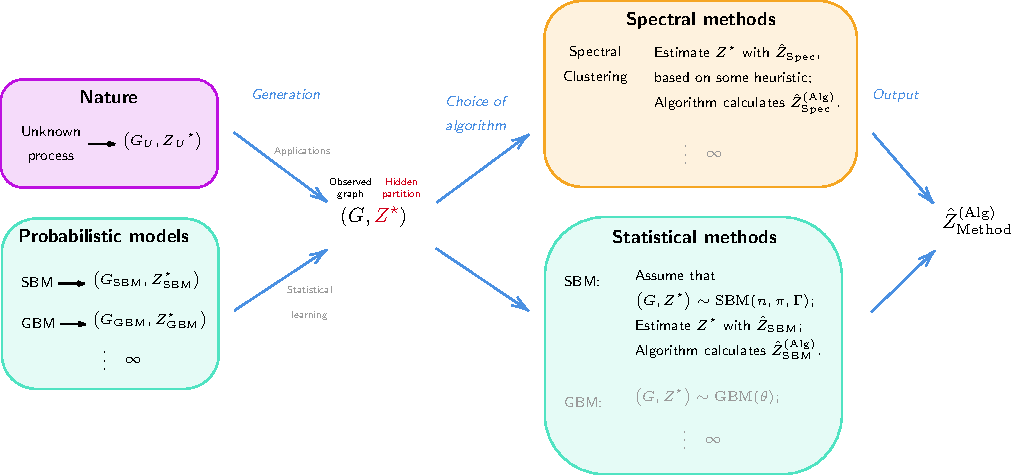
\includegraphics[width=\textwidth]{
				chapters/introduction/images/tikz/diagram-introduction/diagram-introduction.pdf
			}
		\end{adjustbox}
	}{		
		\includegraphics{example-image-a}
	}
	\caption{Steps taken from observing a graph to estimating its communities. 
	First, either an unknown process or some probabilistic model generates a 
	graph, which is observed, and a community assignment on it, which is 
	hidden (not observed). Then, an algorithm is picked to estimate the 
	communities. This report presents two different approaches, namely spectral 
	and statistical, to develop of such algorithms.}
	\label{fig:diagram-introduction}
\end{figure}

\end{document}

